\documentclass[a4paper,12pt]{article}
\usepackage[utf8]{inputenc}

% Mise en page
\textwidth 16cm
\textheight 24cm
\topmargin -1 cm
\oddsidemargin 0cm
\evensidemargin 0cm

\usepackage{amsmath,amssymb,amsthm}
\usepackage{mathabx}
\usepackage{xcolor}
\usepackage[round]{natbib}
\usepackage{enumerate}
\usepackage{hyperref}
\usepackage{array}
\usepackage{graphicx}

% custom colors
\newcommand{\noir}[1]{\textcolor[gray]{0}{#1}}   %% black
\newcommand{\gris}[1]{\textcolor[gray]{0.5}{#1}}
\newcommand{\gray}[1]{\textcolor[gray]{0}{\text{#1}}}
\newcommand{\grey}[1]{\textcolor[gray]{0.5}{\text{#1}}} %% light-gray


%opening
\title{Tree Evaluation and Robustness Testing}
\author{Mahendra Mariadassou$^1$ \and Avner Bar-Hen$^2$ \and Hirohisa Kishino$^3$}
\date{%
$^1$INRA, France\\%
$^2$CNAM, France\\%
$^3$University of Tokyo, Japan%
}

%%%%%%%%%%%%%%%%%%%%%%%%%%%%%%%%%%%%%%%%%%%%%%%%%%%%%%%%%%%%%%%%%%%%%%
%%%%%%%%%%%%%%%%%%%%%%%%%%%%%%%%%%%%%%%%%%%%%%%%%%%%%%%%%%%%%%%%%%%%%
\begin{document}
%%%%%%%%%%%%%%%%%%%%%%%%%%%%%%%%%%%%%%%%%%%%%%%%%%%%%%%%%%%%%%%%%%%%%%
%%%%%%%%%%%%%%%%%%%%%%%%%%%%%%%%%%%%%%%%%%%%%%%%%%%%%%%%%%%%%%%%%%%%%%

\maketitle

\begin{abstract}
Reconstructing phylogenies has become a common task in comparative biology. It is however difficult to construct fully reliable phylogenies: trees estimated from different loci may differ and different genetic characters may support different phylogenies. Validation and robustness assessment are therefore critical. Here, we review sources of errors and uncertainties and introduce support values used to characterize weak and strong parts of the tree. We also show to construct robust consensus trees from a robust and how to detect outliers at either the loci or species level. Finally, we show how continuous distances on a tree space can be used to frame validation in a statistical setting.
\end{abstract}

\tableofcontents

%%%%%%%%%%%%%%%%%%%%%%%%%%%%
%%%%%%%%%%%%%%%%%%%%%%%%%%%%
\section{Motivation} \label{sec:Motivation}

%%%%%%%%%%%%%%%%%%%%%%%%%%%%
\subsection{Applications of Phylogenies} \label{sec:applications}

Molecular phylogenetics is a lively field of research with a number of practical applications. 
Reconstructing large phylogenies, such as the bird [ref] or mammal phylogeny [ref], is of intrinsic interest 
to evolutionary biologists, but those phylogenies also \emph{the basic structures necessary to think clearly about differences between species, and to analyze those differences statistically}~\citep{Felsenstein2004}. They arise frequently in comparative genomics, conservation issues~\citep{Bordewich2008}, functional prediction of genes~\citep{Eisen1998} and more generally are at the heart of Phylogenetic Comparative Methods~\citep{Revell2008, Pennell2013}. Most, if not all, applications of phylogenetics have in common that they rely on accurate phylogenetic estimates and it is crucial to validate the tree as different trees can lead to vastly different conclusions (\emph{e.g.} one ancestral emergence of a phenotypic trait versus many independent ones [ref]).  

With the advent of molecular data and increased formalism of the field~\citep{Gascuel2005a}, modern phylogenetic reconstruction is now essentially a statistical inference problem. Many popular reconstruction softwares such as PhyML~\citep{Guindon2003}, RAxML~\citep{Stamatakis2006}, FastTree~\citep{Price2010} or MrBayes~\citep{Ronquist2003} produce a statistical estimate of the tree and we also frame validation in a statistical framework. We first discuss the different sources of inaccuracies in the reconstructed tree (Section~\ref{sec:error-sources}) and distinguish between natural variability ($\simeq$ variance) and modeling errors ($\simeq$ bias). We then briefly describe and discuss popular support values (Section~\ref{sec:robustness}) aimed at validating a tree. The variability, when expressed as a forest of trees, can be summarized in order to produce confidence sets and robust tree estimates (Section~\ref{sec:confidence}). Finally, we review promising developments in the field of robustness validation (Section~\ref{sec:extensions})

% We distinguish to natural uncertainty, due to lack of signal in the data, and other sources of inaccuracies, arising for example from erroneous sequence alignments, misspecified evolution models, etc. 

%%%%%%%%%%%%%%%%%%%%%%%%%%%%
\subsection{Validating the Tree} \label{sec:tree-validation}

Many inference methods return a single focal tree on  and validation is most often concerned with it. A tree is a complex object that encodes the evolutionary relationship of a set of species. There are two families of validation methods based on (i) the scale at which validation is performed and (ii) whether the tree is considered alone or with respect to other trees. 

\begin{itemize}
 \item The first family is \textbf{local} and grounded on the observation that a tree is uniquely determined by its branches. A tree can thus be validated by computing a \emph{support value} for each of its branch. Support values tell us which parts of the tree are \emph{reliable}, in a yet to be defined way. 
 \item The second family is \textbf{global} and considers the focal tree as a whole. It compares it to a set of alternatives using statistical tests. The tests tell us whether the tree is strictly better (\emph{i.e.} a better fit to the molecular data) than the alternatives. 
\end{itemize}

The two approaches have a different focus but are complimentary. In particular, testing the focal tree against alternatives derived from it can be used to compute support values. 

%%%%%%%%%%%%%%%%%%%%%%%%%%%%
\subsection{Robust Estimate} \label{sec:robust-estimate}

Most softwares return the best tree for a given criteria (\emph{e.g.} likelihood for PhyML and RAxML). Support values tell us whether the tree is reliable and tests tell us whether it's much better than second best or other alternatives. 

In the presence of outlier data, the best tree may be very sensitive to a few data points: slight changes in the molecular data may dramatically change the best tree, with deep clades moving from one position in the tree to another~\citep{Bar-Hen2008}. Since molecular data are inherently noisy, it is interesting to produce \textbf{robust} trees that nearly, but not completely, optimize the criteria while being resilient to small changes in the molecular data. 

A straighforward way to build a robust estimate is to start from a forest of \emph{good} trees and summarize them in some way to build a \textbf{consensus} tree. The forest can consist of trees that are only slightly worse than the best tree (\emph{e.g} bayesian consensus) or that are inferred from slightly perturbed data (\emph{e.g.} bootstrap consensus). 

%%%%%%%%%%%%%%%%%%%%%%%%%%%%
%%%%%%%%%%%%%%%%%%%%%%%%%%%%
\section{Sources of Error} \label{sec:error-sources}

%We do not address the species tree/gene tree discrepancy.
%
%\begin{itemize}
% \item Sampling errors
% \item Modeling errors
%\end{itemize}
Genome analysis indicate that a substantial fraction of genes yield phylogenies that are in strong conflict with one another Broadly speaking, these conflicts derive from two sources: (i) The inability of traditional phylogenetic reconstruction methods to deal with the complexity of molecular evolution on the largest scale (methodological sources) and/or (ii) Real biological events such as lateral gene transfer (LGT) of whole genes between genomes or transfer of subgene fragments within and between genomes (biological sources).

Methodological factors affecting phylogenetic reconstruction include the choice of optimality criterion, limited data availability, taxon sampling and specific assumptions in the modelling of sequence evolution. Biological processes such as the action of natural selection or genetic drift may cause the history of the genes under analysis to obscure the history of the taxa. The large number of potential explanations for the presence of incongruence in molecular phylogenetic analyses makes decisions on how to handle conflict in larger sets of molecular data difficult \cite{rokas2003genome}
%%%%%%%%%%%%%%%%%%%%%%%%%%%%
\subsection{Biological Errors} \label{sec:sampling-error}
%Noisy data (imperfect alignments, sequencing error, one individual per species, different parts of the gene/genome can have different evolutionary histories).

Biologial source of errors are very diverse and among other we may cite  contamination,  frameshift  events,  incorrect  annotations,  erroneous  chimerical  sequences,  wrong orthology assessment, horizontal gene transfer, gene conversion, incomplete lineage sorting or hybridization, etc. (see \cite{philippe2017pitfalls} for example)

Due to the limitations of ancient sequencing technologies, sequencing errors were frequent and sequence quality was quite variable in these early datasets. High-throughput  sequencing  has  greatly  improved  sequence  quality,  mainly  through  the  large  coverage  of each nucleotide, but has simultaneously flooded researchers with an amount of data that is  impossible to  handle  by  hand. The most frequent errors observed are sequencing errors (especially for transcriptomic data) and annotation errors (especially for genomic data).  Errors due to the inclusion of non-orthologous sequences in phylogenomics can have drastic consequences on the final results (\cite{laurin2012origin,philippe2011resolving}).  Contamination is not the only source of non-orthology, paralogy being a common underhand source of issues, given the high frequency of gene/genome duplication, gene conversion and gene loss. Sequence contamination can occurr at the sampling step or at the laboratory or sequencing steps (cross-contamination).

The importance of a correct alignment in phylogenetic inference has long been pointed out (\cite{morrison1997effects,ogden2006multiple,talavera2007improvement,wong2008alignment}). Yet, due to the lack of a tractable model of sequence evolution in the presence of insertion and deletion events (indels), the criteria optimized by alignment software are mostly ad hoc  and based on the simplistic assumptions that homologous characters should be similar and that indels are rare events.

%%%%%%%%%%%%%%%%%%%%%%%%%%%%
%\subsection{Limited Amount of Informations} \label{sec:small-n}
%Noisy data (imperfect alignments, sequencing error, one individual per species, different parts of the gene/genome can have different evolutionary histories).

%%%%%%%%%%%%%%%%%%%%%%%%%%%%
\subsection{Modeling Errors} \label{sec:modeling-errors}
%Site independence
%
%%%%%%%%%%%%%%%%%%%%%%%%%%%%%
%\subsubsection{Model Misspecification} \label{sec:misspecification}
%Use of oversimplified models (Rokas et al).

Every model is only a rough approximation to the reality of molecular evolution. At first, the assumption of independent and identical evolutionary forces across sites is certainly not true in reality. What happens at one site will depend quite critically on where that site lies in a protein or structural RNA. One approach that has been developed is to allow the rate of evolution to vary across the sites (\cite{goldman1994codon}). In essence the rate at the site is introduced into the model as a random effect from a given distribution (often a gamma distribution). \cite{felsenstein1996hidden} extended this approach to allow the rate to depend on the rate at the neighbouring sites along the sequence using a hidden Markov model. This model is expected to work well if most autocorrelation of sites occurs at neighbouring positions in the linear sequence. However, the situation in real molecules is more complex than this with serial dependence not expected as the main type of dependence.. 

The rate matrices used for amino acid substitutions (JTT or PAM)are derived by averaging over patterns observed in thousands of sites. However it is clear (\cite{halpern1998evolutionary,parisi2001structural,susko2002testing}) that amino acid frequencies at sites strongly deviate from the frequencies expected under the JTT matrix.  Lartillot and Philippe (\cite{lartillot2004bayesian}) implemented a Bayesian mixture model which allows the inference of site specific rate matrices. These studies indicate that relaxing the assumption that all sites evolve according to the same rate matrices is of key importance for accurate phylogenetic inference from proteins. However, it seems likely that serious, difficult to diagnose, problems stemming from over-parameterization could result from the extremely parameter-rich models (see \cite{rannala2002identifiability} for a  discussion of over-parameterization of phylogenetic models in the context of Bayesian inference).

Most models  assume stationarity, homogeneity and reversibility of the stochastic process of sequence change, even though it has been clear for many years that these assumptions are violated when considering the evolutionary process over very long time scales \citep{boussau2006efficient}. For instance, the set of nucleotide or amino acid positions free to vary, and the evolutionary rates at which they vary, and the frequencies of nucleotides, codons and amino acids can periodically change over the tree, due to functional or structural alterations in the molecule or differing selective forces in the organisms' genomes.

Other cases where the homogeneity, stationarity and/or time-reversibility of substitution models are violated include situations where the underlying state frequencies (whether they be nucleotides, amino acids or codons) in the genes of different organisms vary over the tree. If distantly related lineages begin to display similar state frequencies, these lineages can be artefactually grouped together (see for example \cite{foster2004modeling,jermiin2004biasing}). Finally, non-vertical transmission and more generally non-reticulated evolution is best captured by phylogenetic networks rather than phylogenetic trees \citep{huson2005application}. 

% Clearly the existence of lateral gene transfer (LGT) is a major deviation form the standard model of vertical descent. Approaches are being developed to incorporate LGT into evolutionary models of genomes (see \cite{zhaxybayeva2004genome} for example).
%%%%%%%%%%%%%%%%%%%%%%%%%%%%
% \subsubsection{Complex Evolutionary History} \label{sec:complex-history}

% Incomplete Lineage Sorting (in a multi tree Context)  %%1 page %% ABH

%%%%%%%%%%%%%%%%%%%%%%%%%%%%
%%%%%%%%%%%%%%%%%%%%%%%%%%%%
\section{Robustness} \label{sec:robustness}

As discussed in Section~\ref{sec:Motivation}, support values are a popular way to validate a focal tree. We present here the most popular ones before describing other methods to validate or enhance a tree. 

%%%%%%%%%%%%%%%%%%%%%%%%%%%%
\subsection{Support Values} \label{sec:confidence-values}

%%%%%%%%%%%%%%%%%%%%%%%%%%%%
\subsubsection{Bootstrap} \label{sec:bootstrap}

Bootstrap values~\cite{Felsenstein1985} are probably the most popular and easiest to understand support values. Bootstrap involves resampling from one's molecular data with to create fictional datasets, called \emph{bootstrap replicates}, of the same size. Specifically, the molecular data is typically organized as a multiple sequence alignment (MSA) of $s$ species $\times$ $n$ characters. Since most models assume independent characters, we generate a replicate by sampling $n$ characters, with replacement, from the original MSA and do this $B$ times. Note that in each replicate, some characters are sampled more than once and some left out entirely. The $B$ replicates are used to estimate a forest of $B$ bootstrap trees (one per replicate). Finally the bootstrap value ($BP$) of a branch of the original tree is its frequency of occurrence in the forest. The process is illustrated in Figure~\ref{fig:bootstrap}. 

\begin{figure}
  \begin{center}
	\begin{tabular}{>{\centering\arraybackslash}m{4cm}cc}
	  \textbf{MSA} & & \textbf{Inferred Tree} \\
	  %% Original data
	  & \\
	  \multicolumn{3}{c}{Original Data}\\
	  $
	  \begin{array}{|c|cccc|}
	    \hline
	    \textbf{A} & \noir{A} & \gris{C} & \gray{T} & \grey{T} \\
	    \textbf{B} & \noir{G} & \gris{G} & \gray{A} & \grey{T} \\
	    \textbf{C} & \noir{G} & \gris{G} & \gray{C} & \grey{C} \\
	    \hline
	  \end{array}
	  $
	  &
	  $\longrightarrow$
	  &
	  \begin{minipage}[c]{0.25\linewidth}
	    \begin{center}
	      
\includegraphics[width=0.6\linewidth]{Figs/TrueOne3.pdf}
	    \end{center}
	  \end{minipage} 
	  \\
	  %% Replicate 1
	  & \\
	  \multicolumn{3}{c}{Bootstrap Replicate \#1}\\
	  $
	  \begin{array}{|c|cccc|}
	    \hline
	    \textbf{A} & \noir{A} & \gris{C} & \gray{T} & \gris{C} \\
	    \textbf{B} & \noir{G} & \gris{G} & \gray{A} & \gris{G} \\
	    \textbf{C} & \noir{G} & \gris{G} & \gray{C} & \gris{G} \\
	    \hline
	  \end{array}
	  $
	  &
	  $\longrightarrow$
	  &
	  \begin{minipage}[c]{0.25\linewidth}
	    \begin{center}
	      
\includegraphics[width=0.6\linewidth]{Figs/TrueOne1.pdf}
	    \end{center}
	  \end{minipage}
	  \\
          %% Replicate 2
	  & \\
	  \multicolumn{3}{c}{Bootstrap Replicate \#2}\\
	  $
          \begin{array}{|c|cccc|}
            \hline
            \textbf{A} & \gris{C} & \noir{A} & \gray{T} & \noir{A} \\
            \textbf{B} & \gris{G} & \noir{G} & \gray{A} & \noir{G} \\
            \textbf{C} & \gris{G} & \noir{G} & \gray{C} & \noir{G} \\
            \hline
          \end{array}
          $
          &
          $\longrightarrow$
          &
          \begin{minipage}[c]{0.25\linewidth}
            \begin{center}
              
\includegraphics[width=0.6\linewidth]{Figs/TrueOne1.pdf}
            \end{center}
          \end{minipage}
          \\
          %% Replicate 3
	  & \\
	  \multicolumn{3}{c}{Bootstrap Replicate \#3}\\
	  $
          \begin{array}{|c|cccc|}
            \hline
            \textbf{A} & \gray{T} & \grey{T} & \grey{T} & \gray{T} \\
            \textbf{B} & \gray{A} & \grey{T} & \grey{T} & \gray{A} \\
            \textbf{C} & \gray{C} & \grey{C} & \grey{C} & \gray{C} \\
            \hline
          \end{array}
	  $
          &
          $\longrightarrow$
          &
          \begin{minipage}[c]{0.25\linewidth}
            \begin{center}
              
\includegraphics[width=0.6\linewidth]{Figs/TrueOne2.pdf}
            \end{center}
          \end{minipage}
          \\
	\end{tabular}
   \end{center}
   \caption{Principle of the bootstrap for phylogenies. Each character is identified by its color and style. Characters are sampled with replacement to produce bootstrap replicates, which are then used to infer phylogenies. The split $A|BC$ appears in $2$ out of $3$ bootstrap trees and therefore has a bootstrap value of $BP = 2/3$ or $66$\%.}
  \label{fig:bootstrap}
\end{figure}

Intuitively, the variation obtained by resampling $n$ sites from the original data should be the same as the variation obtained by sampling $n$ new characters. Bootstrap values capture, among other, the \emph{sampling} variability induced short MSA. When $n$ increases, so does $BP$ in general and it is quite common to achieve very high values for all branches when working on genome-scale alignments~\citep{Rokas2003}. 

$BP$ provides a guide for the amount of support a branch has: branches with high $BP$ occur more often and are more reliable than those with low $BP$. Although it might be tempting to interpret $BP$ as the probability that a branch is present in the (unknown) true tree, this is not the case in general. \cite{Zharkikh1992} showed in a simple case that $BP$ is biased and underestimates that probability. Using simulation studies, \cite{Hillis1993} showed that $BP$ values as small as 70\% could reflect highly supported branches. Many studies~\citep{Felsenstein1993, Efron1996, Susko2008, Susko2010} examined the theoretical properties of bootstrap values and concluded that they are indeed biased. This bias is partly induced by the peculiar geometry of tree space (see \cite{Billera2001, Susko2010} and Section~\ref{sec:extensions}). 

The final limitation of bootstrap values, shared with other support values based on resampling techniques, is that they are quite computationally expensive to compute: the budget required to compute $B$ bootstrap trees is $B$-fold higher than the one required to compute the original tree. Clever implementations can substantially reduce that cost~\citep{Stamatakis2014} but it remains prohibitive for very large trees. 

%%%%%%%%%%%%%%%%%%%%%%%%%%%%
\subsubsection{Posterior Probabilities} \label{sec:posterior-probabilities}

Posterior Probabilities ($PP$) are mostly used in a Bayesian framework and similar in spirit bootstrap values. The main difference lies in the forest of trees used to compute support values. Bayesian procedures estimate the posterior distribution of trees. In practice, the distribution is too complex to fully explore and software produce a Markov Chain Markov Chains (MCMC) sample the posterior distribution~\citep{Yang1997a}. The $PP$ of a branch is computed, just like $BP$, as the the probability of occurrence of that branch in the MCMC sample. MCMC trees constitute a set of highly likely trees (best, second best, etc) for the original dataset. $PP$ are easier to interpret than $BP$ as they approximate directly the probability that a branch is present in the true tree, given the original data. Furthermore, since MCMC trees are a natural byproduct of the estimation procedure, there is almost no overhead in computing $PP$. 

Unfortunately, $PP$ are not immune to bias. Empirical studies found that $PP$ are generally higher than $BP$~\citep{Anisimova2011} and sometimes even overconfident. The ``star-tree paradox'' \citep{Yang2007} is the most extreme example of spurious support. \citet{Yang2007} showed that when the actual tree is a 3 species star-like, with no real inner branch, and that sequence length goes to $\infty$, one branch randomly chosen among the 3 potential but erroneous inner branches, has its $PP$ that goes to $100$\% whereas one would expect all potential branches to have $PP$ around $33$\%. 

Intuitively, $PP$ are higher than $BP$ because they cover fewer sources of variability. Unlike bootstrap trees, MCMC trees all originate from the same dataset. $PP$ are quite good at capturing the lack of phylogenetic signal in the original MSA but not the impact of a few influential characters. For example, outlier characters with a strong effect on tree inference will affect all MCMC trees consistently. By contrast, they will be included in some replicates but left out from others leading to more variation among bootstrap trees than among MCMC trees. Finally, in genome-scale context where inaccuracies are more likely to arise from modeling errors than from sampling variability, $PP$ are uniformly high and as uninformative as $BP$~\citep{Philippe2011, Kumar2012}

%%%%%%%%%%%%%%%%%%%%%%%%%%%%
\subsubsection{Likelihood-based Support Values} \label{sec:other-confidence}

Both $BP$ and $PP$ quantify the agreement between a focal tree and forest of trees. Likelihood-based supports are fast alternatives that bypass the forest and deal exclusively with the focal tree~\citep{Anisimova2006}. 

For any inner branch, there are NNI configurations around that branch: the focal one $T_1$ and two alternatives $T_2$, $T_3$ (see see Figure~\ref{fig:nni}). If we note $\ell_i = \log Pr(D \| T_i)$ the likelihood of the data under tree $i$ and assume that $T_1$ is the maximum-likelihood tree, we have $\ell_1 \geq \max(\ell_2, \ell_3)$. Likelihood-based supports values essentially test whether $\delta = \ell_1 - \max(\ell_2, \ell_3)$ is significantly larger than $0$. 

\begin{figure}
 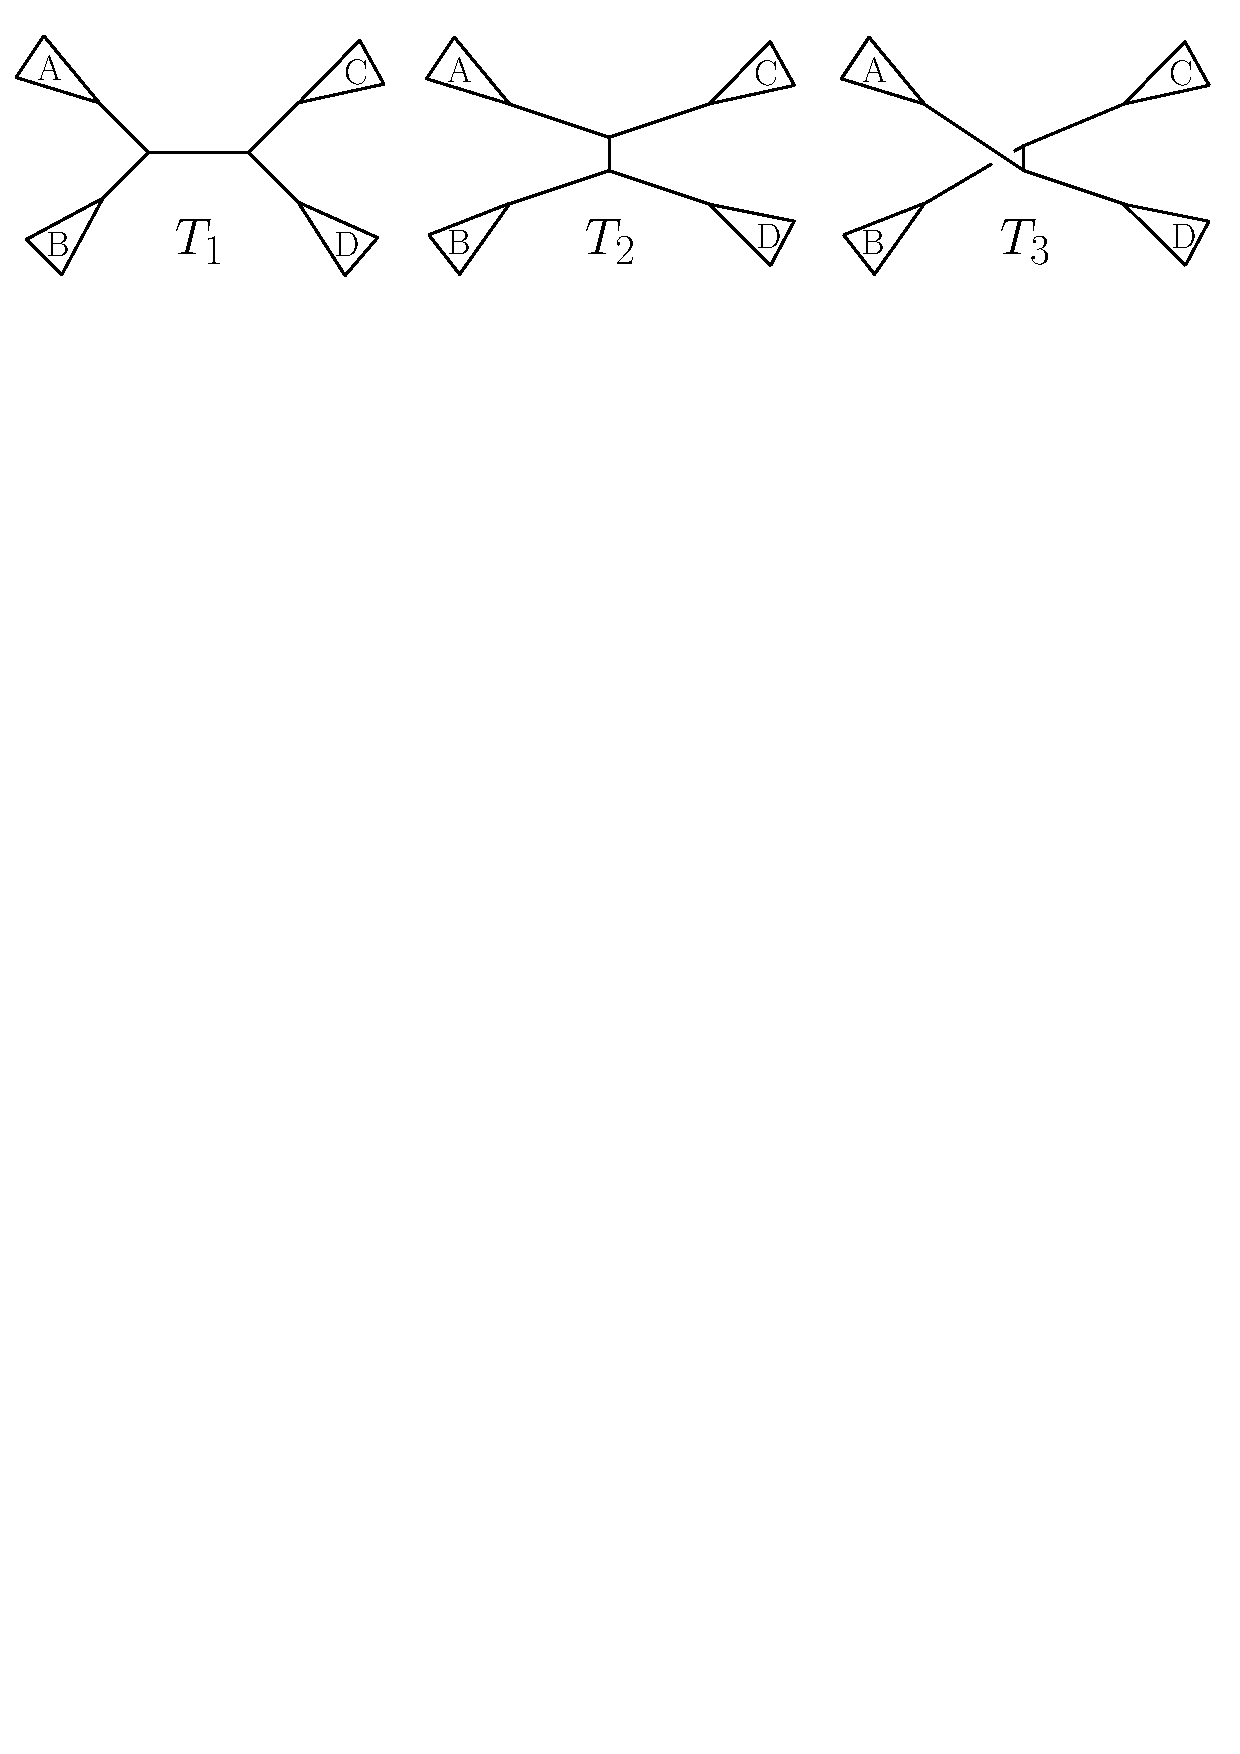
\includegraphics[width=0.9\linewidth]{Figs/NNI}
 \caption{The maximum likelihood tree ($T_1$, left) and its two NNI-alternatives ($T_{2}$ middle and $T_{3}$ right) corresponding to different resolutions of the inner branch. Subtrees are sketched as triangles.}
 \label{fig:nni}
\end{figure}


The most popular support values are:
\begin{itemize}
 \item the approximate Likelihood Ratio Tests (aLRT) values which evaluates the statistics $\delta$ and compares it to $0.5\chi^2_0 + 0.5\chi^2_1$ to compute a p-value. The p-value is then converted into a support value between $1/8$ and $1$. A branch with high $\delta$ will have high support. 
 \item the SH-corrected aLRT (SH-aLRT) values are based on the same idea but use the non-parametric~\citet{Shimodaira1999} procedure to compute the p-value of $\delta$.
 \item Finally approximate bayes (aBayes) is an approximation of the posterior probability of tree $T_i$ computed as:
 \[
  Pr(T_i | D) = \frac{Pr(T_i) Pr(D | T_i)}{\sum_{j=1}^3 Pr(T_j) Pr(D | T_j)}
 \]
 with a flat prior $Pr(T_1) = Pr(T_2)= Pr(T_3)$
\end{itemize}

All likelihood-based supports (aBayes, aLRT, SH-aLRT) amount to testing if $T_1$ is significantly better than $T_2$ and $T_3$. By focusing on one branch at the time rather than questioning the whole tree, likelihood-based supports are less conservative than $BP$ and $PP$. They can also reuse likelihood computed while estimating the focal tree and are therefore much faster to compute than standard $BP$. Finally, they proved to be accurate in simulations studies~\citep{Anisimova2011}. They are the default support values in PhyML~\citep{Guindon2003}. 

%%%%%%%%%%%%%%%%%%%%%%%%%%%%
\subsection{Outliers in the Data} \label{sec:outliers}

The aforementioned support values aggregate all variations in the data set and are unable to distinguish between genuine and spurious variations due to outliers. The nature of resampling techniques is to use the empirical distribution as a surrogate for the true distribution. However, the empirical distribution may be polluted by outliers, defined here as ``entry in the data set that are anomalous with respect to
the behavior seen in the majority of the other entries in the data set''~\citep{Barnett1994}. This is a common occurrence in multi-locus studies where some characters can evolve according to one a tree, and others according to another tree~\cite{Degnan2009}. In that case, a single phylogeny is not a good fit to all the characters and~\citet{Swofford1996} argued that it should be interesting to pinpoint where the phylogeny is not a good fit of the molecular data. Restricting the analyses to congruent characters usually leads to higher support values~\citep{Bar-Hen2008}.
%%%%%%%%%%%%%%%%%%%%%%%%%%%%
% \subsubsection{Rogue Sites} \label{sec:rogue-sites}

Many diagnostic approaches have been developed to identify outlier characters. Many studies \citep{Rodriguez-Ezpeleta2007, Burleigh2004} advocate removing fast-evolving characters which are a well-known cause of misleading phylogenetic signal and long branch attraction (LBA) where distantly related taxa are grouped together in the tree due to parallel or convergent evolution. \citet{Lopez1999} also suggest to investigate and remove characters with high rate variations (\emph{i.e.} fast-evolving in some parts of the tree, slow-evolving in others). However both methods rely on good topologies to estimate rates, leading to a circularity problem. 

\citet{Bar-Hen2008} adapted instead influence functions~\citep{Hampel1974} to phylogenetics in order to assess the impact of a single site on the likelihood. The main idea consists in removing one character at a time, to create \emph{jackknife} replicates, and to infer a tree on each replicate. Jackknife trees are used to find influential characters, whose removal most affect the tree likelihood. \citet{Bar-Hen2008} report that influential sites have a strong impact on the topology and correspond mostly to fast evolving sites. All approaches found that removing outliers leads to more stable phylogenies but none is available as a routine in popular softwares. 

%%%%%%%%%%%%%%%%%%%%%%%%%%%%
\subsection{Taxon Sampling} \label{sec:rogue-taxa}

In phylogenomics studies, it is common to have conflicting trees with support values higher than $95$\% for all inner branches~\citep{Rydin2002}. This correspond to setups where the estimated tree has a very small variance and differences between trees result from bias and modeling errors. In particular, \citet{Swofford1996} argues that adequate taxon sampling is one of the primary factors for accurate phylogenetic estimates, on par with enough sequence data. For example, dense taxon sampling can reduce the impact of LBA by splitting long branches ~\citep{Felsenstein1978}. Similarly, \citet{Holland2003} and \citet{Shavit2007} showed that the inclusion of an outgroup to the analysis may disrupt the ingroup phylogeny. When there are only a few taxa, but many characters, phylogenetic analysis can produce high support values ($BP$, $PP$, etc.) for incorrect or misleading phylogenies~\citep{Rokas2003, Rokas2005, Heath2008}.

Analysis of sensitivity to taxon inclusion should be a part of careful and thorough phylogenetic analysis~\citep{Heath2008}. \citet{Mariadassou2012} defined a the Taxon Influence Index (TII) to assess the influence of each on the phylogeny. Using any inference method, we define $T^*$ to be the tree inferred from the complete MSA. Let $T_k$ be a smaller tree, inferred from the
alignment deprived of taxon $k$ and $T_k^*$ the tree obtained by pruning taxon $k$ from $T^*$. 
The TII is the distance between trees $T_k$ and $T_k^*$, such that 
\[
TII(k) = d(T_k , T_k^*) 
\]
They found that most taxa have small TII(k) and little influence on the topology whereas a few are highly influential \emph{rogue taxa} and alter the phylogeny in clades even loosely related to their placement in the tree. \citet{Aberer2013} use a different approach, they start from a forest of trees (\emph{e.g.} bootstrap trees) and search for a small set of taxa whose pruning increases the agreement between trees in the forest. The method is implemented in the webservice RogueNarok. Both methods find that pruning rogue taxa improves accuracy and results in more stable phylogenies with higher support values. 

%%%%%%%%%%%%%%%%%%%%%%%%%%%%
%%%%%%%%%%%%%%%%%%%%%%%%%%%%
\section{Confidence Sets} \label{sec:confidence}

Summarize a forest of tree
\begin{itemize}
 \item Consensus Tree
 \item Confidence Set
\end{itemize}

%%%%%%%%%%%%%%%%%%%%%%%%%%%%
\subsection{Consensus Tree} \label{sec:consensus-tree}

Different methods for a consensus (and problems in terms of branch lengths reconstruction)

%%%%%%%%%%%%%%%%%%%%%%%%%%%%
\subsection{Confidence Set} \label{sec:confidence-sets}

Easy to understand in a Bayesian setting, a bit more involved (AIC weights) in a frequentist framework. 
 %3 pages %% MM

% %%%%%%%%%%%%%%%%%%%%%%%%%%%%
%%%%%%%%%%%%%%%%%%%%%%%%%%%%
\section{Testing} \label{sec:testing}

Likelihood based tests for 
\begin{itemize}
 \item topology against topology (or topologies)
 \item model against model
 \item node/branch against polytomy (=branch length)
\end{itemize}

%%%%%%%%%%%%%%%%%%%%%%%%%%%%
\subsection{Likelihood Based Tests} \label{sec:likelihood-tests}
KH, SH, AU

%%%%%%%%%%%%%%%%%%%%%%%%%%%%
\subsection{Model Testing} \label{sec:model-test}
model test

%%%%%%%%%%%%%%%%%%%%%%%%%%%%
\subsection{Node Testing} \label{sec:node-test}
Test polytomy using using nested models and LRT. Bayes factor in a Bayesian setting.

%%%%%%%%%%%%%%%%%%%%%%%%%%%%
%%%%%%%%%%%%%%%%%%%%%%%%%%%%
\section{Detection of conflicting signal} \label{sec:extensions}

Consensus trees assumes congruence among trees in the set. Trees that turn out to be far away from the consensus tree can be the sign of high variance or conflicting signals. While high variance implies weak phylogenetic signal, conflicting  signals implies incongruence. Most distance distances, such as RF, are discrete and lead to very coarse distance distributions. By contrast, continuous distances are a simple way to characterize variance and distinguish one from the other. Moreover continuous distance lend themselves nicely to standard aspects of inferential statistics such as confidence sets and hypothesis testing. 

%Consider the space tree
%\begin{itemize}
% \item BHV space topology
% \item Means and variances in the tree space \textcolor{red}{briefly mentioned in previous section}
% \item Multivariate Analysis based on tree distances
% \end{itemize}

The  geometric  model of \cite{Billera2001} allows one to compare phylogenetic  trees,  with  the  same  leaf  set  of  cardinality $m$, in a quantitative way.  This  space  has  a  natural  metric, giving a way of measuring distance between phylogenetic trees and providing some procedures for averaging or combining several trees whose leaves are identical. This geometry also shows which trees appear within a fixed distance of a given tree and enables construction of convex hulls of a
set of trees. It also provides a justification for disregarding portions of a collection of trees that agree,  thus simplifying the space in which comparisons are to be made.

%%%%%%%%%%%%%%%%%%%%%%%%%%%%
\subsection{Tree Space definition} \label{sec:Tree-distances}
 The distance $d(T_i,T_j)$ between two trees $T_i$ and $T_j$ account for differences with respect to both their tree topologies (branching structure) and branch lengths. The space is constructed by representing each of the $(2m-3)!!$ possible tree topologies by a single non-negative Euclidean orthant of dimension $m-3$ (the largest possible number of internal branches). The orthants are then “glued together” along appropriate axes. Specifically, nearest neighbor interchange (NNI) topologies lie in adjacent non-negative orthants along the boundary corresponding to the collapse of the relevant NNI edge.

For two trees with different topologies, the BHV distance is the length of the shortest path between them that remains in the treespace.  The length of any path can be computed by calculating the Euclidean distance of the path restricted to each orthant that it passes though, and summing these lengths.  The shortest path is called a geodesic, and will pass from one orthant to the next orthant through lower-dimensional boundaries corresponding to trees with fewer splits. Since the space is nonpositively  curved, the geodesics are unique. 

\begin{figure}
 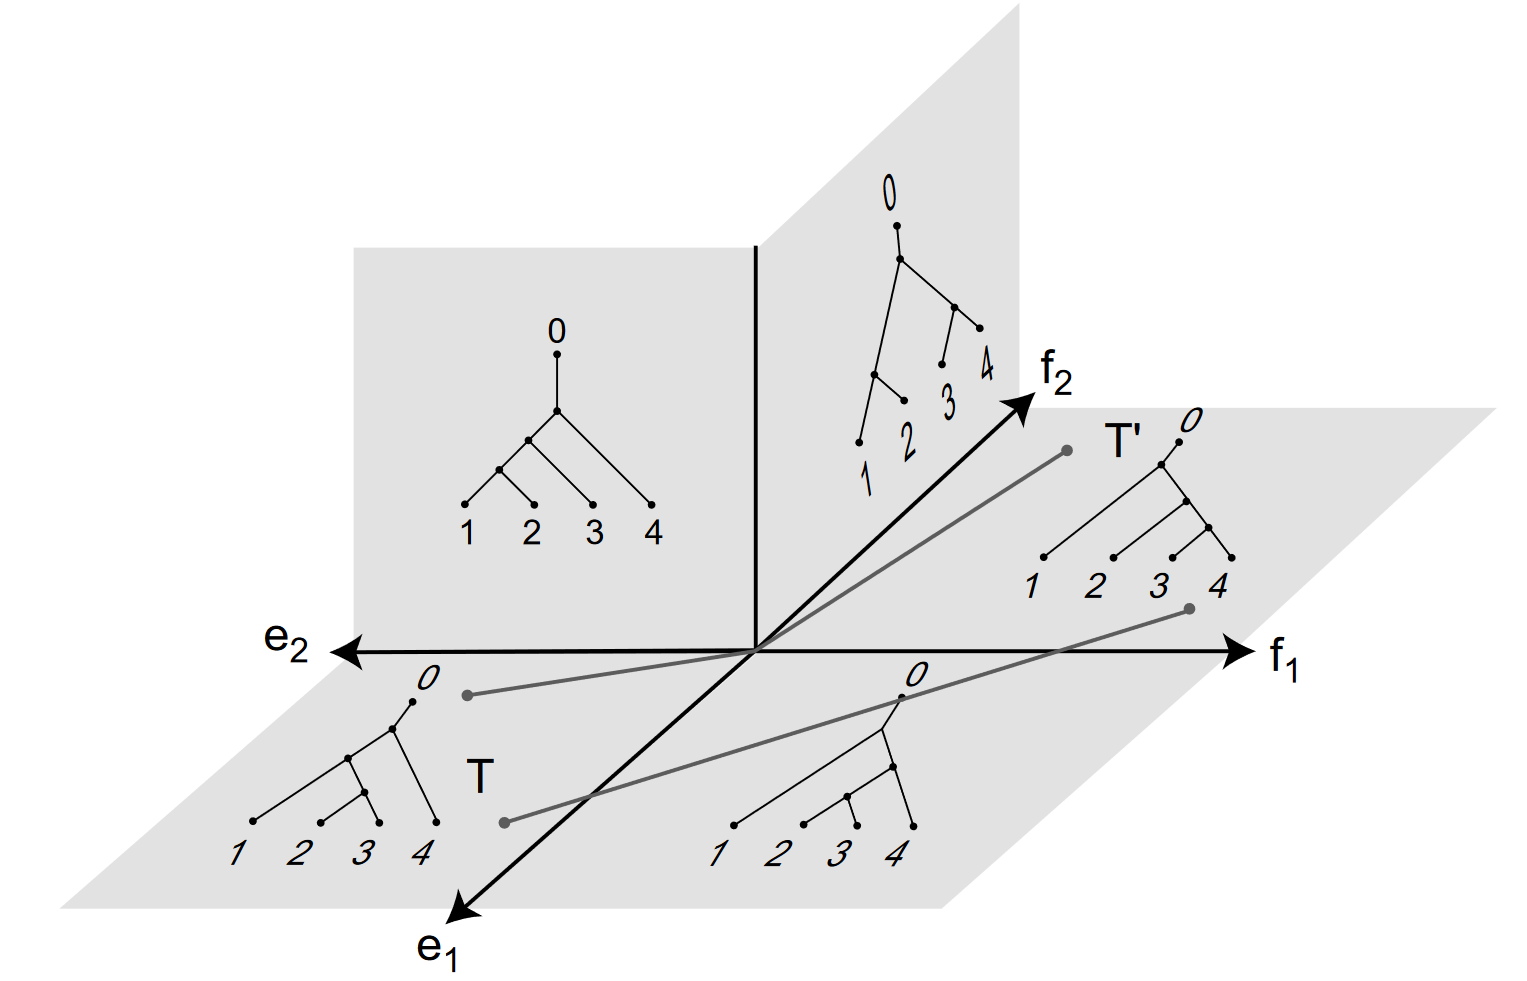
\includegraphics{Figs/OrthantBHV}
 \caption{Orthants in the BHV space (one per topology) and geodesic paths between two trees corresponding to topologies $T$ and $T'$. Reproduced from \citet{Billera2001}.}
\end{figure}

In Euclidean space, the Fr\'echet mean is the point minimizing the sum of the squared distances to the sample points, and is equivalent to the coordinate-wise average of the sample points. The mean tree is not necessarily a refinement of the majority-rule consensus tree. Fr\'echet variance is the tree that minimize the sum of squared distances.  This variance is unique because treespace is non-positively curved. The Fr\'echet variance of a set of trees quantifies how spread out a set of trees is from their mean. See \cite{miller2015polyhedral,brown2017mean} for details.

%%%%%%%%%%%%%%%%%%%%%%%%%%%%
\subsection{Use of BHV distance} \label{sec:means-and-variance}

\cite{barden2017logarithm} proved a Central Limit Theorem on the BHV treespace, showing that the distribution of the sample means converges to a certain Gaussian distribution. It is useful for detecting splits of weak and strong support and in tree-valued hypothesis testing.

A key tool of \cite{barden2014limiting}is  the log map  that permits to  map  trees  from  their  metric  space  to  Euclidean space, where it is possible to model a tree estimate $\hat T$ as a noisy realization of the true tree $T$. Once  the model parameters are estimated, Euclidean multivariate analysis techniques to reduce the dimension of the trees can be used. This allows to visualize tree estimates, along with their uncertainties.

For example it is possible to use the variance covariance matrix to  estimate  the  principal  directions  of  variability  via principal components analysis. The axes of the $\mathbb{R}^m$ ellipsoid indicate the relative directions of precision, and the ellipsoid can be shrunk  to be wholly contained in the same orthant as $\hat T_n$. This gives an unambiguous indication of the relative
confidence in the edges of the estimated tree. Note that the procedure is unambiguous about the trees contained in the confidence set for a given confidence level $\alpha$ (see \cite{willis2016confidence}).

Recently, \cite{de2012phylo} developed a statistical non-parametric method to detect outlier trees from the set of gene trees. They first convert gene trees into vectors in a multidimensional Euclidean space and then apply multiple co-inertia analysis (MCOA)—an extension of principal coordinate analysis—directly to these vectorized gene trees. Their method, Phylo-MCOA, also detects outlier species, those whose position varies widely from tree to tree. Included in our results are simulation studies comparing our non-parametric method with Phylo-MCOA.

\cite{weyenberg2014kdetrees}  proposes  a non-parametric estimator of the distribution that generated the sample trees $T_1,\ldots,T_n$.  This estimator can be viewed as a refined version of histogram-based estimation of a density. The kernel function, is a non-negative function defined on pairs of trees, which measures how similar two trees are. Kernel density estimation use the fact that points close to sample points tend to have higher likelihood than distant outlier points.  The ultimate goal is to detect outlier trees, $T_j$, which are not actually drawn from the true distribution.
%%%%%%%%%%%%%%%%%%%%%%%%%%%%
%\subsection{Confidence Sets Based on other Distances} \label{sec:kernel}
%
%Kernel based methods (using a distance matrix) to find outlier and build confidence sets.

%%%%%%%%%%%%%%%%%%%%%%%%%%%%
\subsection{Need for a Strong Theoretical Framework} 

With the democratization of high-throughput sequencing, acquiring new genome data has ceased to be the limiting factor in phylogenetic, except maybe for organisms that are difficult to sample from the environment. In contrast, phylogeneticists are now faced with a rise in data errors, which stems from a flood of increasingly bogus genomic data that has become intractable by hand. Given the size of current and upcoming phylogenomic datasets (thousands of genes for hundreds —   and soon thousands —   of species), computational requirements are emerging as the new limiting factor. As multiple possible improvements are theoretically able to limit systematic error (and artefacts) during phylogenetic inference, we  need  to determine the set of properties that the ideal model of sequence of evolution should combine.  An alternative approach is to use robustness methods to downweight or discard portions of the data where model misspecification occurs potentially mitigating the estimation biases these data may incur. This latter, in combination with improved models, may ultimately allow the development of robust and efficient analytical
tools that are also computationally tractable.  %1 - 2 pages %% ABH

\section{Further Reading}

Interested readers can refer to 
\begin{itemize}
 \item \citet{Felsenstein2004} to very broad introduction to phylogenetics;
 \item \citet{Susko2010} for an in-depth analysis of the bias in bootstrap values and potential corrections;
 \item \citet{Bryant2003} for a extensive review of consensus methods and their mathematical properties;
 \item \citet{St.John2017} for a extensive review of distances between trees;
 \item \citet{Yang2007} for a detailed analysis of the star tree paradox and problem with posterior probabilities in phylogenetics;
 \item \citet{Degnan2009} for a primer on the gene tree / species tree problem;
 \item \citet{philippe2017pitfalls} for the pitfalls of phylogenomics.
\end{itemize}

\bibliographystyle{plainnat}
\bibliography{robustness}

%%%%%%%%%%%%%%%%%%%%%%%%%%%%%%%%%%%%%%%%%%%%%%%%%%%%%%%%%%%%%%%%%%%%%%
%%%%%%%%%%%%%%%%%%%%%%%%%%%%%%%%%%%%%%%%%%%%%%%%%%%%%%%%%%%%%%%%%%%%%%
\end{document}
%%%%%%%%%%%%%%%%%%%%%%%%%%%%%%%%%%%%%%%%%%%%%%%%%%%%%%%%%%%%%%%%%%%%%%
%%%%%%%%%%%%%%%%%%%%%%%%%%%%%%%%%%%%%%%%%%%%%%%%%%%%%%%%%%%%%%%%%%%%%% 